\documentclass{article}


\usepackage{PRIMEarxiv}

\usepackage[utf8]{inputenc} % allow utf-8 input
\usepackage[T1]{fontenc}    % use 8-bit T1 fonts
\usepackage{hyperref}       % hyperlinks
\usepackage{url}            % simple URL typesetting
\usepackage{booktabs}       % professional-quality tables
\usepackage{amsfonts}       % blackboard math symbols
\usepackage{nicefrac}       % compact symbols for 1/2, etc.
\usepackage{microtype}      % microtypography
\usepackage{lipsum}
\usepackage{fancyhdr}       % header
\usepackage{graphicx}       % graphics
\graphicspath{{media/}}     % organize your images and other figures under media/ folder

\usepackage{amsmath,amssymb}
\usepackage{algorithmic}
\usepackage{algorithm}
\usepackage{textcomp}
\usepackage{xcolor}
\usepackage{multirow}
\usepackage{cite}

%Header
\pagestyle{fancy}
\thispagestyle{empty}
\rhead{ \textit{ }} 

% Update your Headers here
%\fancyhead[LO]{SELF-LEARNING MIXTURE OF EXPERTS WITH ICA-BASED
%INITIALIZATION FOR ENHANCED EEG ARTIFACT REMOVAL}
% \fancyhead[RE]{Firstauthor and Secondauthor} % Firstauthor et al. if more than 2 - must use \documentclass[twoside]{article}



  
%% Title
\title{Self-Learning Mixture of Experts with ICA-Based Initialization for Enhanced EEG Artifact Removal
%%%% Cite as
%%%% Update your official citation here when published 
%\thanks{\textit{\underline{Citation}}: 
%\textbf{Authors. Title. Pages.... DOI:000000/11111.}} 
}

\author{
  Ping Liang \\
  Department of Electronics Engineering \\
  Batangas State University \\
  Batangas, Philippines \\
  \texttt{22-07901@g.batstate-u.edu.ph} \\
  %% examples of more authors
   \And
  Anton Louise De Ocampo \\
  Department of Electronics Engineering \\
  Batangas State University \\
  Batangas, Philippines \\
  \texttt{antonlouise.deocampo@g.batstate-u.edu.ph} \\
  %% \AND
  %% Coauthor \\
  %% Affiliation \\
  %% Address \\
  %% \texttt{email} \\
  %% \And
  %% Coauthor \\
  %% Affiliation \\
  %% Address \\
  %% \texttt{email} \\
  %% \And
  %% Coauthor \\
  %% Affiliation \\
  %% Address \\
  %% \texttt{email} \\
}
\begin{document}
\maketitle


\begin{abstract}
Electroencephalography (EEG) signals are frequently contaminated by physiological artifacts, including electrooculography (EOG) and electromyography (EMG) artifacts, which significantly degrade the quality of neural recordings and subsequent analyses. Mixture of Experts (MoE) architectures offer promising adaptability through specialized expert networks, but a fundamental challenge is achieving meaningful expert specialization without explicit artifact labels---experts often converge to similar solutions (mode collapse), negating the benefits of the modular architecture. In this paper, we propose a novel \textbf{Self-Learning ICA-Initialized Mixture of Experts (ICA-MoE)} framework that addresses this challenge through an innovative ICA-based self-learning pre-training strategy. Our key contribution is using Independent Component Analysis (ICA) to automatically characterize signal components by their spectral content and statistical properties (skewness, kurtosis), then leveraging these characteristics to create expert-specific training targets that guide each expert toward distinct specializations---low-frequency neural components, high-frequency artifacts, non-Gaussian artifact sources, and ensemble refinement. This self-learning initialization eliminates the need for manual artifact labeling while ensuring complementary expert behaviors. The framework employs a gating network that routes inputs to appropriate experts based on learned ICA features, with load balancing regularization to maintain stable expert utilization. Comprehensive experiments on real EEG, EOG, and EMG datasets demonstrate that our ICA-MoE approach achieves superior denoising performance, significantly outperforming state-of-the-art deep learning baselines. The self-learning ICA initialization proves essential---without it, experts converge to similar outputs and performance degrades substantially.
\end{abstract}


% keywords can be removed
\keywords{Mixture of Experts \and Independent Component Analysis \and Self-learning initialization \and EEG artifact removal \and Expert specialization \and Deep learning}

%=====================================================================
\section{Introduction}
\label{sec:introduction}

Electroencephalography (EEG) has become an indispensable tool in neuroscience research, brain-computer interfaces (BCIs), and clinical diagnostics due to its non-invasive nature and high temporal resolution \cite{teplan2002fundamentals, niedermeyer2005electroencephalography}. However, EEG signals are inherently susceptible to various physiological and non-physiological artifacts that can severely compromise signal quality and the validity of downstream analyses \cite{uriguen2015eeg}. Among physiological artifacts, electrooculography (EOG) artifacts caused by eye movements and blinks, and electromyography (EMG) artifacts arising from muscle activity, are particularly prevalent and challenging to remove due to their spectral overlap with neural signals of interest \cite{fatourechi2007emg, jiang2019removal}.

Traditional artifact removal approaches can be broadly categorized into regression-based methods, filtering techniques, and blind source separation (BSS) algorithms \cite{islam2016methods}. Regression-based methods, such as least mean squares (LMS) and recursive least squares (RLS) adaptive filters, require clean reference signals and assume linear relationships between artifacts and EEG \cite{he2004removal}. Independent Component Analysis (ICA), a popular BSS technique, has been widely adopted for artifact identification and removal but typically requires manual component selection and is sensitive to non-stationarity \cite{jung2000removing, delorme2004eeglab}. Recent deep learning approaches, including convolutional neural networks (CNNs) and recurrent neural networks (RNNs), have shown promise in learning artifact patterns directly from data \cite{yang2018automatic, zhang2021eegdenoisenet}. However, these methods often employ monolithic architectures that lack adaptability to varying artifact characteristics.

The Mixture of Experts (MoE) paradigm has emerged as a powerful architectural framework in machine learning, particularly in natural language processing and computer vision \cite{shazeer2017outrageously, fedus2022switch}. MoE architectures employ multiple specialized expert networks, each focusing on different aspects of the input space, combined through a gating mechanism that learns to route inputs to the most appropriate experts \cite{jacobs1991adaptive}. This conditional computation approach offers several advantages: improved model capacity without proportional computational cost, enhanced interpretability through expert specialization, and adaptive processing based on input characteristics \cite{riquelme2021scaling}.

A fundamental challenge in applying MoE to EEG artifact removal is achieving meaningful expert specialization. Without proper initialization, experts tend to converge to similar solutions---a phenomenon known as representation collapse \cite{chi2022collapse}---which negates the benefits of the modular architecture. Simply training an MoE end-to-end often fails to produce the diverse, complementary expert behaviors needed for effective artifact removal.

However, hard-coded initialization requires initial knowledge about the frequency bands of the EEG signal: $\delta$ (0.5-4 Hz), $\theta$ (4-7 Hz), $\alpha$ (8-12 Hz), $\sigma$ (12-16 Hz), and $\beta$ (13-30 Hz) \cite{nayak2025waves}. To optimize the results of this method needs numerous manual adjustment of the initialized parameters, which motivates the self-learning initialization in this paper. 

In this paper, we propose a novel \textbf{Self-Learning ICA-Initialized Mixture of Experts (ICA-MoE)} framework that addresses this challenge through an innovative ICA-based self-learning pre-training strategy. Our key contributions are as follows:

\begin{enumerate}
\item \textbf{Self-Learning ICA-Based Expert Initialization (Primary Contribution)}: We introduce a novel self-learning pre-training strategy that leverages ICA component characteristics to automatically create expert-specific training targets \textit{without requiring manual artifact labels}. By analyzing ICA components' spectral content (low/high frequency power ratios) and statistical properties (skewness, kurtosis), we guide each expert toward distinct specializations: Expert 0 for low-frequency neural components, Expert 1 for high-frequency content, Expert 2 for non-Gaussian artifact sources, and Expert 3 for ensemble refinement. This initialization is crucial---it prevents mode collapse and enables the complementary expert behaviors that make MoE effective.

\item \textbf{ICA-Enhanced Feature Representation}: We augment the input features with real-time ICA component characteristics computed via sliding window decomposition. These features provide the gating network with rich signal characterization, enabling more informed expert routing decisions.

\item \textbf{Independence-Promoting Training}: We incorporate an independence loss during pre-training that explicitly penalizes correlation between expert outputs, further encouraging diverse specialization and preventing expert collapse.

\item \textbf{Comprehensive Evaluation}: We conduct extensive experiments demonstrating that the ICA-based initialization is essential for performance---the same MoE architecture without our initialization strategy shows degraded results, validating the importance of our self-learning approach.
\end{enumerate}

The remainder of this paper is organized as follows: Section \ref{sec:related_work} reviews related work on EEG artifact removal and MoE architectures. Section \ref{sec:methodology} presents our proposed ICA-MoE framework in detail. Section \ref{sec:experiments} describes the experimental setup and evaluation metrics. Section \ref{sec:results} presents the experimental results and comparisons. Section \ref{sec:discussion} discusses the implications and limitations of our approach. Finally, Section \ref{sec:conclusion} concludes the paper and outlines future research directions.

%=====================================================================
\section{Related Work}
\label{sec:related_work}

\subsection{EEG Artifact Removal Methods}

EEG artifact removal has been extensively studied over the past decades. \textbf{Regression-based methods} model artifacts as linear combinations of reference signals. The Least Mean Squares (LMS) algorithm \cite{widrow1975adaptive} iteratively updates filter coefficients to minimize the mean squared error between the estimated and actual signals. The Recursive Least Squares (RLS) algorithm \cite{haykin2014adaptive} provides faster convergence by utilizing all past data samples. Kalman filtering approaches \cite{morbidi2008application} model the EEG signal as a state-space system and recursively estimate the clean signal.

\textbf{Blind source separation (BSS)} methods, particularly Independent Component Analysis (ICA), have become standard tools for EEG artifact removal \cite{jung2000removing}. ICA decomposes multichannel EEG into statistically independent components, allowing artifact components to be identified and removed. FastICA \cite{hyvarinen1999fast} and Infomax ICA \cite{bell1995information} are widely used algorithms. However, ICA requires multichannel recordings and manual component selection, limiting its applicability in single-channel or automated systems.

\textbf{Deep learning approaches} have recently gained attention for EEG denoising. Zhang et al. \cite{zhang2021eegdenoisenet} proposed EEGDnoiseNet, a dilated convolutional network with residual connections for artifact removal. Autoencoders and variational autoencoders have been applied to learn latent representations of clean EEG signals \cite{yang2018automatic}. Recurrent architectures, including Long Short-Term Memory (LSTM) networks, capture temporal dependencies in EEG data \cite{lawhern2018eegnet}. Despite their effectiveness, these methods typically employ fixed architectures that do not adapt to varying artifact characteristics.

\subsection{Mixture of Experts Architectures}

The Mixture of Experts (MoE) model was introduced by Jacobs et al. \cite{jacobs1991adaptive} as a modular approach to supervised learning, where multiple expert networks specialize in different regions of the input space. The gating network learns to weight expert outputs based on input features. Shazeer et al. \cite{shazeer2017outrageously} scaled MoE to thousands of experts for language modeling, introducing sparsely-gated MoE layers that activate only a subset of experts per input.

Recent advances in MoE have demonstrated their effectiveness in various domains. The Switch Transformer \cite{fedus2022switch} simplified MoE routing by selecting only one expert per token, enabling efficient scaling to trillion-parameter models. Vision MoE \cite{riquelme2021scaling} applied sparse MoE to image recognition, achieving competitive performance with reduced computational cost. Mixtral \cite{jiang2024mixtral} combined MoE with the Mistral architecture for improved language understanding.

The key advantages of MoE architectures include: (1) increased model capacity without proportional computational increase through sparse activation, (2) improved generalization through expert specialization, and (3) interpretability through analysis of expert activation patterns \cite{chen2023mixture}. These properties make MoE particularly suitable for EEG artifact removal, where different artifact types may require specialized processing strategies.

Researches on using MoE architecture for EEG denoising are limited. \cite{choi2025moeemg} indicates that the MoE algorithm performs well in routing and removing SNR-varied types of EMG artifacts from EEG signals. 

\subsection{ICA in Neural Network Initialization}

Combining ICA with neural networks has been explored in various contexts. ICA-based feature extraction has been used as preprocessing for neural network classifiers before feeding into deep learning architectures \cite{makeig2004mining} \cite{vw2023} \cite{sutharsan2022}. Some works have used ICA to initialize convolutional filters, improving convergence and performance on image classification tasks \cite{le2011ica}. Recent work \cite{gcmcg2025} has combined ICA preprocessing with MoE architectures for EEG decoding, but the expert specialization is guided by electrode topology rather than ICA component characteristics. To our knowledge, no prior work has used ICA component characteristics to guide the specialization of expert networks in an MoE framework for EEG denoising.

%=====================================================================

\begin{figure*}[!t]
    \centering
    \includegraphics[width=1\linewidth]{fig1.png}
        \caption{Diagram of ICA-Initiated MoE framework. Its features include: I) ICA Decomposition: Extracts 4 independent components using FastICA with window-based processing; II) Self-Learning Pre-training: Experts specialize on different ICA components before main training; III) Expert Specialization: a) Expert 0: Low-frequency components; b) Expert 1: High-frequency components; c)Expert 2: Non-Gaussian artifacts (high kurtosis/skewness); d) Expert 3: Adaptive weighted mixing of all components; IV) Sparse Gating: Top-k=2 routing for computational efficiency; V) Dual-Phase Training: ICA pre-training (5 epochs) followed by main MoE training (10 epochs); VI) Load Balancing: Ensures balanced expert utilization during training}
    \label{fig:architecture}
\end{figure*}


\section{Methodology}
\label{sec:methodology}

\subsection{Problem Formulation}

Let $\mathbf{x}(t) \in \mathbb{R}^T$ denote the observed EEG signal at time $t$, modeled as:
\begin{equation}
\mathbf{x}(t) = \mathbf{s}(t) + \mathbf{a}_{\text{EOG}}(t) + \mathbf{a}_{\text{EMG}}(t) + \mathbf{n}(t)
\end{equation}
where $\mathbf{s}(t)$ is the clean neural signal, $\mathbf{a}_{\text{EOG}}(t)$ represents ocular artifacts, $\mathbf{a}_{\text{EMG}}(t)$ denotes muscular artifacts, and $\mathbf{n}(t)$ is additive noise. Our objective is to estimate $\hat{\mathbf{s}}(t)$ from $\mathbf{x}(t)$ and auxiliary artifact reference signals.

\subsection{System Architecture Overview}

Figure \ref{fig:architecture} illustrates the overall architecture of our ICA-MoE framework, which consists of four main components:

\begin{enumerate}
\item \textbf{ICA Decomposer}: Extracts independent components and their characteristics from input signals.
\item \textbf{Expert Networks}: Multiple specialized LSTM-based networks, each pre-trained to handle specific signal components.
\item \textbf{Sparse Gating Network}: Routes inputs to the most appropriate experts based on ICA features.
\item \textbf{Output Combiner}: Aggregates expert outputs weighted by gating probabilities.
\end{enumerate}

\subsection{ICA-Based Component Analysis}

The ICA Decomposer performs blind source separation to identify underlying signal components. Given a batch of input signals $\mathbf{X} \in \mathbb{R}^{N \times T}$, we apply FastICA \cite{hyvarinen1999fast} to estimate independent components:
\begin{equation}
\mathbf{C} = \mathbf{W}\mathbf{X}
\end{equation}
where $\mathbf{W}$ is the unmixing matrix and $\mathbf{C} \in \mathbb{R}^{K \times T}$ contains $K$ independent components.

For each component $\mathbf{c}_k$, we compute characteristic features including:

\textbf{Spectral Features}: Using the discrete Fourier transform $\mathcal{F}$, we compute the power spectral density:
\begin{equation}
P_k(f) = |\mathcal{F}(\mathbf{c}_k)|^2
\end{equation}

The low-frequency and high-frequency power ratios are:
\begin{equation}
\rho_{\text{low},k} = \frac{\sum_{f < f_c/4} P_k(f)}{\sum_f P_k(f)}, \quad \rho_{\text{high},k} = \frac{\sum_{f > f_c/2} P_k(f)}{\sum_f P_k(f)}
\end{equation}
where $f_c$ is the Nyquist frequency.

\textbf{Statistical Features}: We compute higher-order statistics that capture non-Gaussianity:
\begin{equation}
\gamma_k = \frac{\mathbb{E}[(\mathbf{c}_k - \mu_k)^3]}{\sigma_k^3}, \quad \kappa_k = \frac{\mathbb{E}[(\mathbf{c}_k - \mu_k)^4]}{\sigma_k^4} - 3
\end{equation}
where $\gamma_k$ is skewness and $\kappa_k$ is excess kurtosis.

These component characteristics guide expert specialization during pre-training and provide features for the gating network.

\subsection{ICA-Based Self-Learning Pre-Training}

A key innovation of our approach is the self-learning pre-training strategy that leverages ICA characteristics to create expert-specific training targets. This enables each expert to specialize in handling different aspects of the signal without requiring explicit artifact labels. The fundamental insight is that ICA decomposition naturally reveals signal characteristics---spectral distribution and statistical properties---that correspond to different signal sources (neural activity vs. artifacts), providing a principled basis for guiding expert specialization.

For each expert $e \in \{0, 1, 2, 3\}$, we construct target signals by blending the ground-truth clean signal $\mathbf{s}$ with component-specific reconstructions derived from ICA analysis. We denote the clean signal weight as $\alpha_e$ and the component reconstruction weight as $\beta_e = 1 - \alpha_e$, where these blending coefficients control how strongly each expert is biased toward different signal aspects. The component selection thresholds $\tau_{\text{low}}$, $\tau_{\text{high}}$, $\tau_{\kappa}$, and $\tau_{\gamma}$ determine which ICA components are included in each expert's target construction.

\textbf{Expert 0 (Low-Frequency Specialist)} is designed to focus on preserving slow neural oscillations, which typically occupy the delta (0.5--4 Hz), theta (4--8 Hz), and alpha (8--13 Hz) bands. The target signal emphasizes components with dominant low-frequency power, identified by the criterion $\rho_{\text{low}} > \tau_{\text{low}}$:
\begin{equation}
\mathbf{t}_0 = \alpha_0 \cdot \mathbf{s} + \beta_0 \cdot \text{Reconstruct}(\mathbf{x}, \mathcal{I}_{\text{low}})
\end{equation}
where $\mathcal{I}_{\text{low}} = \{k : \rho_{\text{low},k} > \tau_{\text{low}}\}$ denotes the index set of low-frequency dominant components. The reconstruction operator $\text{Reconstruct}(\mathbf{x}, \mathcal{I})$ projects the signal onto the subspace spanned by selected ICA components.

\textbf{Expert 1 (High-Frequency Specialist)} targets components containing high-frequency content, which often includes EMG artifacts but also beta (13--30 Hz) and gamma (30+ Hz) neural activity. By learning to process these components, this expert becomes adept at distinguishing between high-frequency artifacts and legitimate neural signals:
\begin{equation}
\mathbf{t}_1 = \alpha_1 \cdot \mathbf{s} + \beta_1 \cdot \text{Reconstruct}(\mathbf{x}, \mathcal{I}_{\text{high}})
\end{equation}
where $\mathcal{I}_{\text{high}} = \{k : \rho_{\text{high},k} > \tau_{\text{high}}\}$ identifies components with substantial high-frequency power.

\textbf{Expert 2 (Artifact Specialist)} focuses on non-Gaussian components, which are typically indicative of artifact contamination. Neural signals tend toward Gaussianity due to the central limit theorem (summation of many independent neural sources), while artifacts such as eye blinks produce highly non-Gaussian distributions with pronounced skewness and kurtosis:
\begin{equation}
\mathbf{t}_2 = \mathbf{s} - \lambda_{\text{art}} \cdot (\hat{\mathbf{a}} - \bar{\mathbf{a}})
\end{equation}
where $\hat{\mathbf{a}} = \text{Reconstruct}(\mathbf{x}, \mathcal{I}_{\text{ng}})$ represents the non-Gaussian component reconstruction with $\mathcal{I}_{\text{ng}} = \{k : |\kappa_k| > \tau_{\kappa} \text{ or } |\gamma_k| > \tau_{\gamma}\}$, $\bar{\mathbf{a}}$ is the mean artifact estimate, and $\lambda_{\text{art}}$ controls the artifact suppression strength.

\textbf{Expert 3 (Ensemble Specialist)} integrates information from all components through adaptive weighting, serving as a refinement expert that can correct residual errors from the specialized experts:
\begin{equation}
\mathbf{t}_3 = \alpha_3 \cdot \mathbf{s} + \beta_3 \cdot \sum_k w_k \cdot \text{Reconstruct}(\mathbf{x}, \{k\})
\end{equation}
The component weights $w_k = (1 + |\kappa_k| + |\gamma_k|)^{-1}$ are inversely proportional to the non-Gaussianity measures, assigning higher weights to components more likely to represent clean neural activity.

During pre-training, each expert is optimized independently using a composite loss function that encourages both accurate reconstruction and diverse specialization:
\begin{equation}
\mathcal{L}_{\text{pre}}^{(e)} = \|\mathbf{y}^{(e)} - \mathbf{t}_e\|_2^2 + \lambda_{\text{ind}} \sum_{e' < e} |\text{corr}(\mathbf{y}^{(e)}, \mathbf{y}^{(e')})|
\end{equation}
The first term measures reconstruction fidelity to the expert-specific target, while the second term is an \textbf{independence loss} that explicitly penalizes correlation between different experts' outputs. The coefficient $\lambda_{\text{ind}}$ balances reconstruction accuracy against output diversity, preventing experts from collapsing to similar solutions.

\subsection{Expert Network Architecture}

Each expert network consists of three stages:

\textbf{Feature Extractor}: A two-layer fully connected network with ReLU activation and dropout:
\begin{equation}
\mathbf{h}_{\text{feat}} = \text{Dropout}(\text{ReLU}(\mathbf{W}_1 \mathbf{f} + \mathbf{b}_1))
\end{equation}
where $\mathbf{f} \in \mathbb{R}^7$ concatenates basic features (EEG, EOG, EMG) and 4 ICA features.

\textbf{Temporal Encoder}: An LSTM layer captures temporal dependencies:
\begin{equation}
\mathbf{h}_t, \mathbf{c}_t = \text{LSTM}(\mathbf{h}_{\text{feat},t}, \mathbf{h}_{t-1}, \mathbf{c}_{t-1})
\end{equation}
with hidden size 128.

\textbf{Output Layer}: A linear projection produces the denoised signal estimate:
\begin{equation}
\hat{s}_t^{(e)} = \mathbf{w}_{\text{out}}^\top \mathbf{h}_t + b_{\text{out}}
\end{equation}

We apply Kaiming initialization \cite{he2015delving} for ReLU layers, orthogonal initialization for LSTM weights, and Xavier initialization \cite{glorot2010understanding} for output layers.

\subsection{Sparse Gating Mechanism}

The gating network determines expert routing based on input features. It consists of:

\textbf{Gating LSTM}: Processes the combined feature sequence:
\begin{equation}
\mathbf{g}_t = \text{LSTM}_{\text{gate}}([\mathbf{x}_t, \mathbf{a}_{\text{EOG},t}, \mathbf{a}_{\text{EMG},t}, \mathbf{c}_t])
\end{equation}

\textbf{Gating MLP}: Produces expert logits:
\begin{equation}
\boldsymbol{\ell}_t = \mathbf{W}_2 \text{ReLU}(\mathbf{W}_1 \mathbf{g}_t + \mathbf{b}_1) + \mathbf{b}_2
\end{equation}

\textbf{Sparse Top-$k$ Selection}: To promote computational efficiency and expert specialization, we select only the top-$k$ experts (with $k=2$ in our experiments):
\begin{equation}
\mathbf{p}_t = \text{Normalize}(\text{TopK}(\text{softmax}(\boldsymbol{\ell}_t), k))
\end{equation}

The final output is the weighted combination of active expert outputs:
\begin{equation}
\hat{\mathbf{s}}_t = \sum_{e \in \text{TopK}(k)} p_t^{(e)} \cdot \hat{s}_t^{(e)}
\end{equation}

\subsection{Training Objective}

The complete training objective combines reconstruction loss with load balancing regularization:

\textbf{Reconstruction Loss}: We use Huber loss (Smooth L1) for robustness to outliers:
\begin{equation}
\mathcal{L}_{\text{rec}} = \begin{cases}
\frac{1}{2}(\hat{\mathbf{s}} - \mathbf{s})^2 & \text{if } |\hat{\mathbf{s}} - \mathbf{s}| < 1\\
|\hat{\mathbf{s}} - \mathbf{s}| - \frac{1}{2} & \text{otherwise}
\end{cases}
\end{equation}

\textbf{Load Balancing Loss}: Following \cite{fedus2022switch}, we encourage balanced expert utilization:
\begin{equation}
\mathcal{L}_{\text{lb}} = E^2 \sum_{e=1}^{E} \bar{p}^{(e)} \cdot L^{(e)}
\end{equation}
where $\bar{p}^{(e)}$ is the mean probability assigned to expert $e$ and $L^{(e)}$ is its total load.

\textbf{Total Loss}:
\begin{equation}
\mathcal{L} = \mathcal{L}_{\text{rec}} + \lambda_{\text{lb}} \mathcal{L}_{\text{lb}}
\end{equation}
with $\lambda_{\text{lb}} = 0.01$.

Training uses Adam optimizer \cite{kingma2014adam} with learning rate $10^{-3}$, cosine annealing schedule, and gradient clipping (max norm 1.0).

%=====================================================================
\section{Experimental Setup}
\label{sec:experiments}

\subsection{Dataset}

We evaluate our method on the EEGdenoiseNet benchmark dataset \cite{eegdenoisenet2021} for this study which offers several advantages that align well with our ICA-guided MoE framework: it aggregates data from five independent studies, is specifically optimized for machine learning-based artifact removal, and provides verified ground-truth signals essential for supervised training.

The dataset comprises 4,514 clean EEG segments and 5,598 muscular artifact segments recorded from 67 participants at a 256 Hz sampling rate. Each two-second segment enables synthesis of contaminated EEG signals at controlled signal-to-noise ratios while preserving the corresponding clean reference for quantitative evaluation. This controlled contamination approach is particularly valuable for training and validating our expert network, as it allows systematic assessment of denoising performance across varying types of artifacts as well as different intensities \cite{choi2025moeemg}.

EEGdenoiseNet \cite{eegdenoisenet2021} has become the predominant benchmark in the EEG denoising literature, with numerous recent deep learning methods reporting results on this dataset \cite{choi2025moeemg}. 

Synthetic contamination is created by adding weighted artifact signals:
\begin{equation}
\mathbf{x}_{\text{noisy}} = \mathbf{s}_{\text{clean}} + \alpha (\mathbf{a}_{\text{EOG}} + \mathbf{a}_{\text{EMG}})
\end{equation}
with contamination factor $\alpha = 0.01$.

Three experimental configurations are evaluated:
\begin{enumerate}
\item \textbf{EEG+EOG}: Ocular artifact removal only
\item \textbf{EEG+EMG}: Muscular artifact removal only
\item \textbf{EEG+EOG+EMG}: Combined artifact removal
\end{enumerate}

\subsection{Preprocessing}

All signals undergo z-score normalization per channel:
\begin{equation}
\tilde{\mathbf{x}} = \frac{\mathbf{x} - \mu_{\mathbf{x}}}{\sigma_{\mathbf{x}}}
\end{equation}

Outputs are denormalized for evaluation using stored statistics.

\subsection{Evaluation Metrics}

We employ six complementary metrics to comprehensively evaluate denoising performance, covering both time-domain and frequency-domain aspects. Throughout this section, we denote the ground-truth clean EEG signal as $\mathbf{s} = \{s_t\}_{t=1}^{T}$, the denoised output signal produced by the model as $\hat{\mathbf{s}} = \{\hat{s}_t\}_{t=1}^{T}$, and the total number of time samples as $T$.

\textbf{Root Mean Square Error (RMSE)} quantifies the average magnitude of reconstruction errors in the original signal amplitude units. Lower values indicate better denoising performance:
\begin{equation}
\text{RMSE} = \sqrt{\frac{1}{T}\sum_{t=1}^{T}(\hat{s}_t - s_t)^2}
\end{equation}

\textbf{Relative RMSE (rRMSE)} normalizes the reconstruction error by the signal energy, providing a scale-invariant measure that facilitates comparison across signals with different amplitudes:
\begin{equation}
\text{rRMSE} = \frac{\text{RMSE}}{\sqrt{\frac{1}{T}\sum_{t=1}^{T}s_t^2}}
\end{equation}

\textbf{Pearson Correlation Coefficient} measures the linear relationship between the denoised and clean signals, where $\sigma_{\hat{\mathbf{s}}}$ and $\sigma_{\mathbf{s}}$ denote the standard deviations of the respective signals. A correlation of 1.0 indicates perfect waveform preservation:
\begin{equation}
\text{Corr} = \frac{\text{Cov}(\hat{\mathbf{s}}, \mathbf{s})}{\sigma_{\hat{\mathbf{s}}} \sigma_{\mathbf{s}}}
\end{equation}

\textbf{Signal-to-Noise Ratio (SNR)} expresses the ratio of signal power to residual noise power in decibels. The numerator represents the clean signal energy, while the denominator captures the reconstruction error energy:
\begin{equation}
\text{SNR} = 10 \log_{10}\left(\frac{\sum_t s_t^2}{\sum_t (\hat{s}_t - s_t)^2}\right) \text{ dB}
\end{equation}

\textbf{SNR Improvement ($\Delta$SNR)} measures the gain in signal quality achieved by the denoising process, computed as the difference between output and input SNR values. Positive values indicate successful artifact reduction:
\begin{equation}
\Delta\text{SNR} = \text{SNR}_{\text{output}} - \text{SNR}_{\text{input}}
\end{equation}

\textbf{Spectral Distortion (SD)} evaluates frequency-domain fidelity by comparing the log power spectral densities of the denoised and clean signals across $F$ frequency bins. Here, $P_{\hat{s}}(f)$ and $P_s(f)$ represent the power spectral density of the denoised and clean signals at frequency $f$, respectively. Lower values indicate better preservation of spectral characteristics:
\begin{equation}
\text{SD} = \sqrt{\frac{1}{F}\sum_{f=1}^{F}\left(\log P_{\hat{s}}(f) - \log P_s(f)\right)^2}
\end{equation}

\subsection{Baseline Methods}

We compare our ICA-MoE framework against both traditional signal processing methods and state-of-the-art deep learning approaches to provide a comprehensive evaluation.

Among \textbf{traditional methods}, we evaluate the Least Mean Squares (LMS) adaptive filter \cite{widrow1975adaptive}, which iteratively updates filter coefficients to minimize mean squared error; the Recursive Least Squares (RLS) filter \cite{haykin2014adaptive}, which provides faster convergence by utilizing all past data samples; and the Kalman filter \cite{morbidi2008application}, which models the EEG signal as a state-space system for recursive estimation. These methods represent the classical approaches to adaptive noise cancellation and provide important baselines for comparison.

For \textbf{deep learning methods}, we implement and evaluate several representative architectures. EEGDnoiseNet \cite{zhang2021eegdenoisenet} employs a 10-layer dilated convolutional network with residual connections, designed specifically for EEG denoising. RNN-EEG utilizes a bidirectional LSTM architecture with an attention mechanism to capture temporal dependencies in both forward and backward directions. ResNet-EEG adapts the residual network paradigm to 1D signals using an encoder-decoder structure for signal reconstruction. SimpleCNN serves as a lightweight baseline with a 3-layer convolutional architecture, providing a reference for comparing more complex models.

\subsection{Implementation Details}

The proposed ICA-MoE framework is implemented with a modular architecture comprising four specialized expert networks, each with a hidden dimension of 128 units. The ICA decomposition extracts four independent components from the input signals, providing the spectral and statistical features that guide expert specialization. During inference, the sparse gating mechanism activates only the top-$k$ experts (with $k=2$) for each input, balancing computational efficiency with model expressiveness.

The training procedure consists of two phases: an ICA-guided pre-training phase spanning 5 epochs, during which experts develop their specialized behaviors, followed by a main training phase of 10 epochs for end-to-end optimization. We employ the Adam optimizer \cite{kingma2014adam} with an initial learning rate of $10^{-3}$ and a cosine annealing schedule. Training uses mini-batches of 32 samples with gradient clipping (maximum norm of 1.0) to ensure stable optimization.

To ensure statistical reliability and assess reproducibility, all experiments are repeated with 5 different random seeds (40-44). Results are reported as mean $\pm$ standard deviation across these runs.

%=====================================================================
\section{Results}
\label{sec:results}

\subsection{Overall Performance Comparison}

\begin{table}[!t]
\centering
\caption{RMSE Comparison Under Different Initialization Methods}
\label{tab:rmse_init}
\begin{tabular}{ccc}
\toprule
\textbf{Seed} & \textbf{Self-Learning Initial.} & \textbf{Hardcoded Initial.} \\
\midrule
40 & \textbf{1.46} & \textbf{1.73} \\
41 & \textbf{1.49} & \textbf{1.92} \\
42 & 1.98 & 1.82 \\
43 & \textbf{1.56} & \textbf{1.57} \\
44 & \textbf{1.49} & \textbf{1.52} \\
\bottomrule
\end{tabular}
\end{table}

Table \ref{tab:rmse_init} indicates that the same MoE architecture with our ICA-based self-learning initialization strategy shows substantially upgraded results compared to that with hard-coded initialization which much depends on intial knowledge.

Table \ref{tab:overall_results} presents the comprehensive comparison between our ICA-MoE method and baseline approaches on the combined artifact removal task (EEG+EOG+EMG).



\begin{table*}[!t]
\centering
\caption{Performance Comparison on Combined Artifact Removal (EEG+EOG+EMG). Best results in \textbf{bold}.}
\label{tab:overall_results}
\begin{tabular}{lcccccc}
\toprule
\textbf{Method} & \textbf{RMSE} $\downarrow$ & \textbf{rRMSE} $\downarrow$ & \textbf{Correlation} $\uparrow$ & \textbf{SNR (dB)} $\uparrow$ & \textbf{$\Delta$SNR (dB)} $\uparrow$ & \textbf{Spectral Dist.} $\downarrow$ \\
\midrule
\multicolumn{7}{l}{\textit{Traditional Methods}} \\
LMS Filter & 95.18 $\pm$ 0.00 & 0.416 $\pm$ 0.000 & 0.922 $\pm$ 0.000 & 7.61 $\pm$ 0.00 & -29.40 $\pm$ 0.00 & 0.060 $\pm$ 0.000 \\
RLS Filter & 87.54 $\pm$ 0.00 & 0.383 $\pm$ 0.000 & 0.925 $\pm$ 0.000 & 8.34 $\pm$ 0.00 & -28.68 $\pm$ 0.00 & 0.069 $\pm$ 0.000 \\
Kalman Filter & 96.34 $\pm$ 0.00 & 0.422 $\pm$ 0.000 & 0.917 $\pm$ 0.000 & 7.50 $\pm$ 0.00 & -29.51 $\pm$ 0.00 & 0.519 $\pm$ 0.000 \\
\midrule
\multicolumn{7}{l}{\textit{Deep Learning Methods}} \\
SimpleCNN & 3.32 $\pm$ 0.00 & 0.015 $\pm$ 0.000 & 0.9999 $\pm$ 0.000 & 36.76 $\pm$ 0.01 & -0.25 $\pm$ 0.01 & 0.011 $\pm$ 0.004 \\
EEGDnoiseNet & 4.59 $\pm$ 0.04 & 0.020 $\pm$ 0.000 & 0.9999 $\pm$ 0.000 & 33.95 $\pm$ 0.08 & -3.06 $\pm$ 0.08 & 0.019 $\pm$ 0.003 \\
RNN-EEG & 10.92 $\pm$ 0.21 & 0.048 $\pm$ 0.001 & 0.9989 $\pm$ 0.000 & 26.42 $\pm$ 0.17 & -10.59 $\pm$ 0.17 & 0.020 $\pm$ 0.001 \\
ResNet-EEG & 4.37 $\pm$ 0.21 & 0.019 $\pm$ 0.001 & 0.9998 $\pm$ 0.000 & 34.38 $\pm$ 0.41 & -2.63 $\pm$ 0.41 & 0.025 $\pm$ 0.018 \\
\midrule
\textbf{ICA-MoE (Ours)} & \textbf{1.59 $\pm$ 0.20} & \textbf{0.007 $\pm$ 0.001} & \textbf{0.99998 $\pm$ 0.000} & \textbf{43.19 $\pm$ 0.99} & \textbf{6.18 $\pm$ 0.99} & \textbf{0.005 $\pm$ 0.001} \\
\bottomrule
\end{tabular}
\end{table*}

Our ICA-MoE achieves remarkable performance improvements across all evaluation metrics. The RMSE of 1.59 represents a 52.1\% reduction compared to the best baseline (SimpleCNN: 3.32), demonstrating substantially more accurate signal reconstruction. The correlation coefficient of 0.99998 indicates near-perfect preservation of the original waveform morphology. In terms of SNR, our method achieves 43.19 dB, representing a 6.43 dB improvement over SimpleCNN. Most notably, the SNR improvement of +6.18 dB stands in stark contrast to all deep learning baselines, which show negative values indicating signal degradation rather than enhancement. The spectral distortion of 0.005 confirms that our approach preserves the frequency-domain characteristics of the clean signal better than all alternatives.

Traditional adaptive filters (LMS, RLS, Kalman) perform poorly due to their inability to model complex non-linear relationships between artifacts and EEG signals. Among deep learning methods, SimpleCNN provides a reasonable baseline but fails to achieve positive SNR improvement. RNN-EEG, despite its temporal modeling capability, shows the worst deep learning performance, likely due to gradient vanishing issues. Our ICA-MoE's superior performance stems from the synergy between ICA-based component analysis and adaptive expert routing.

\begin{figure}[!t]
    \centering
    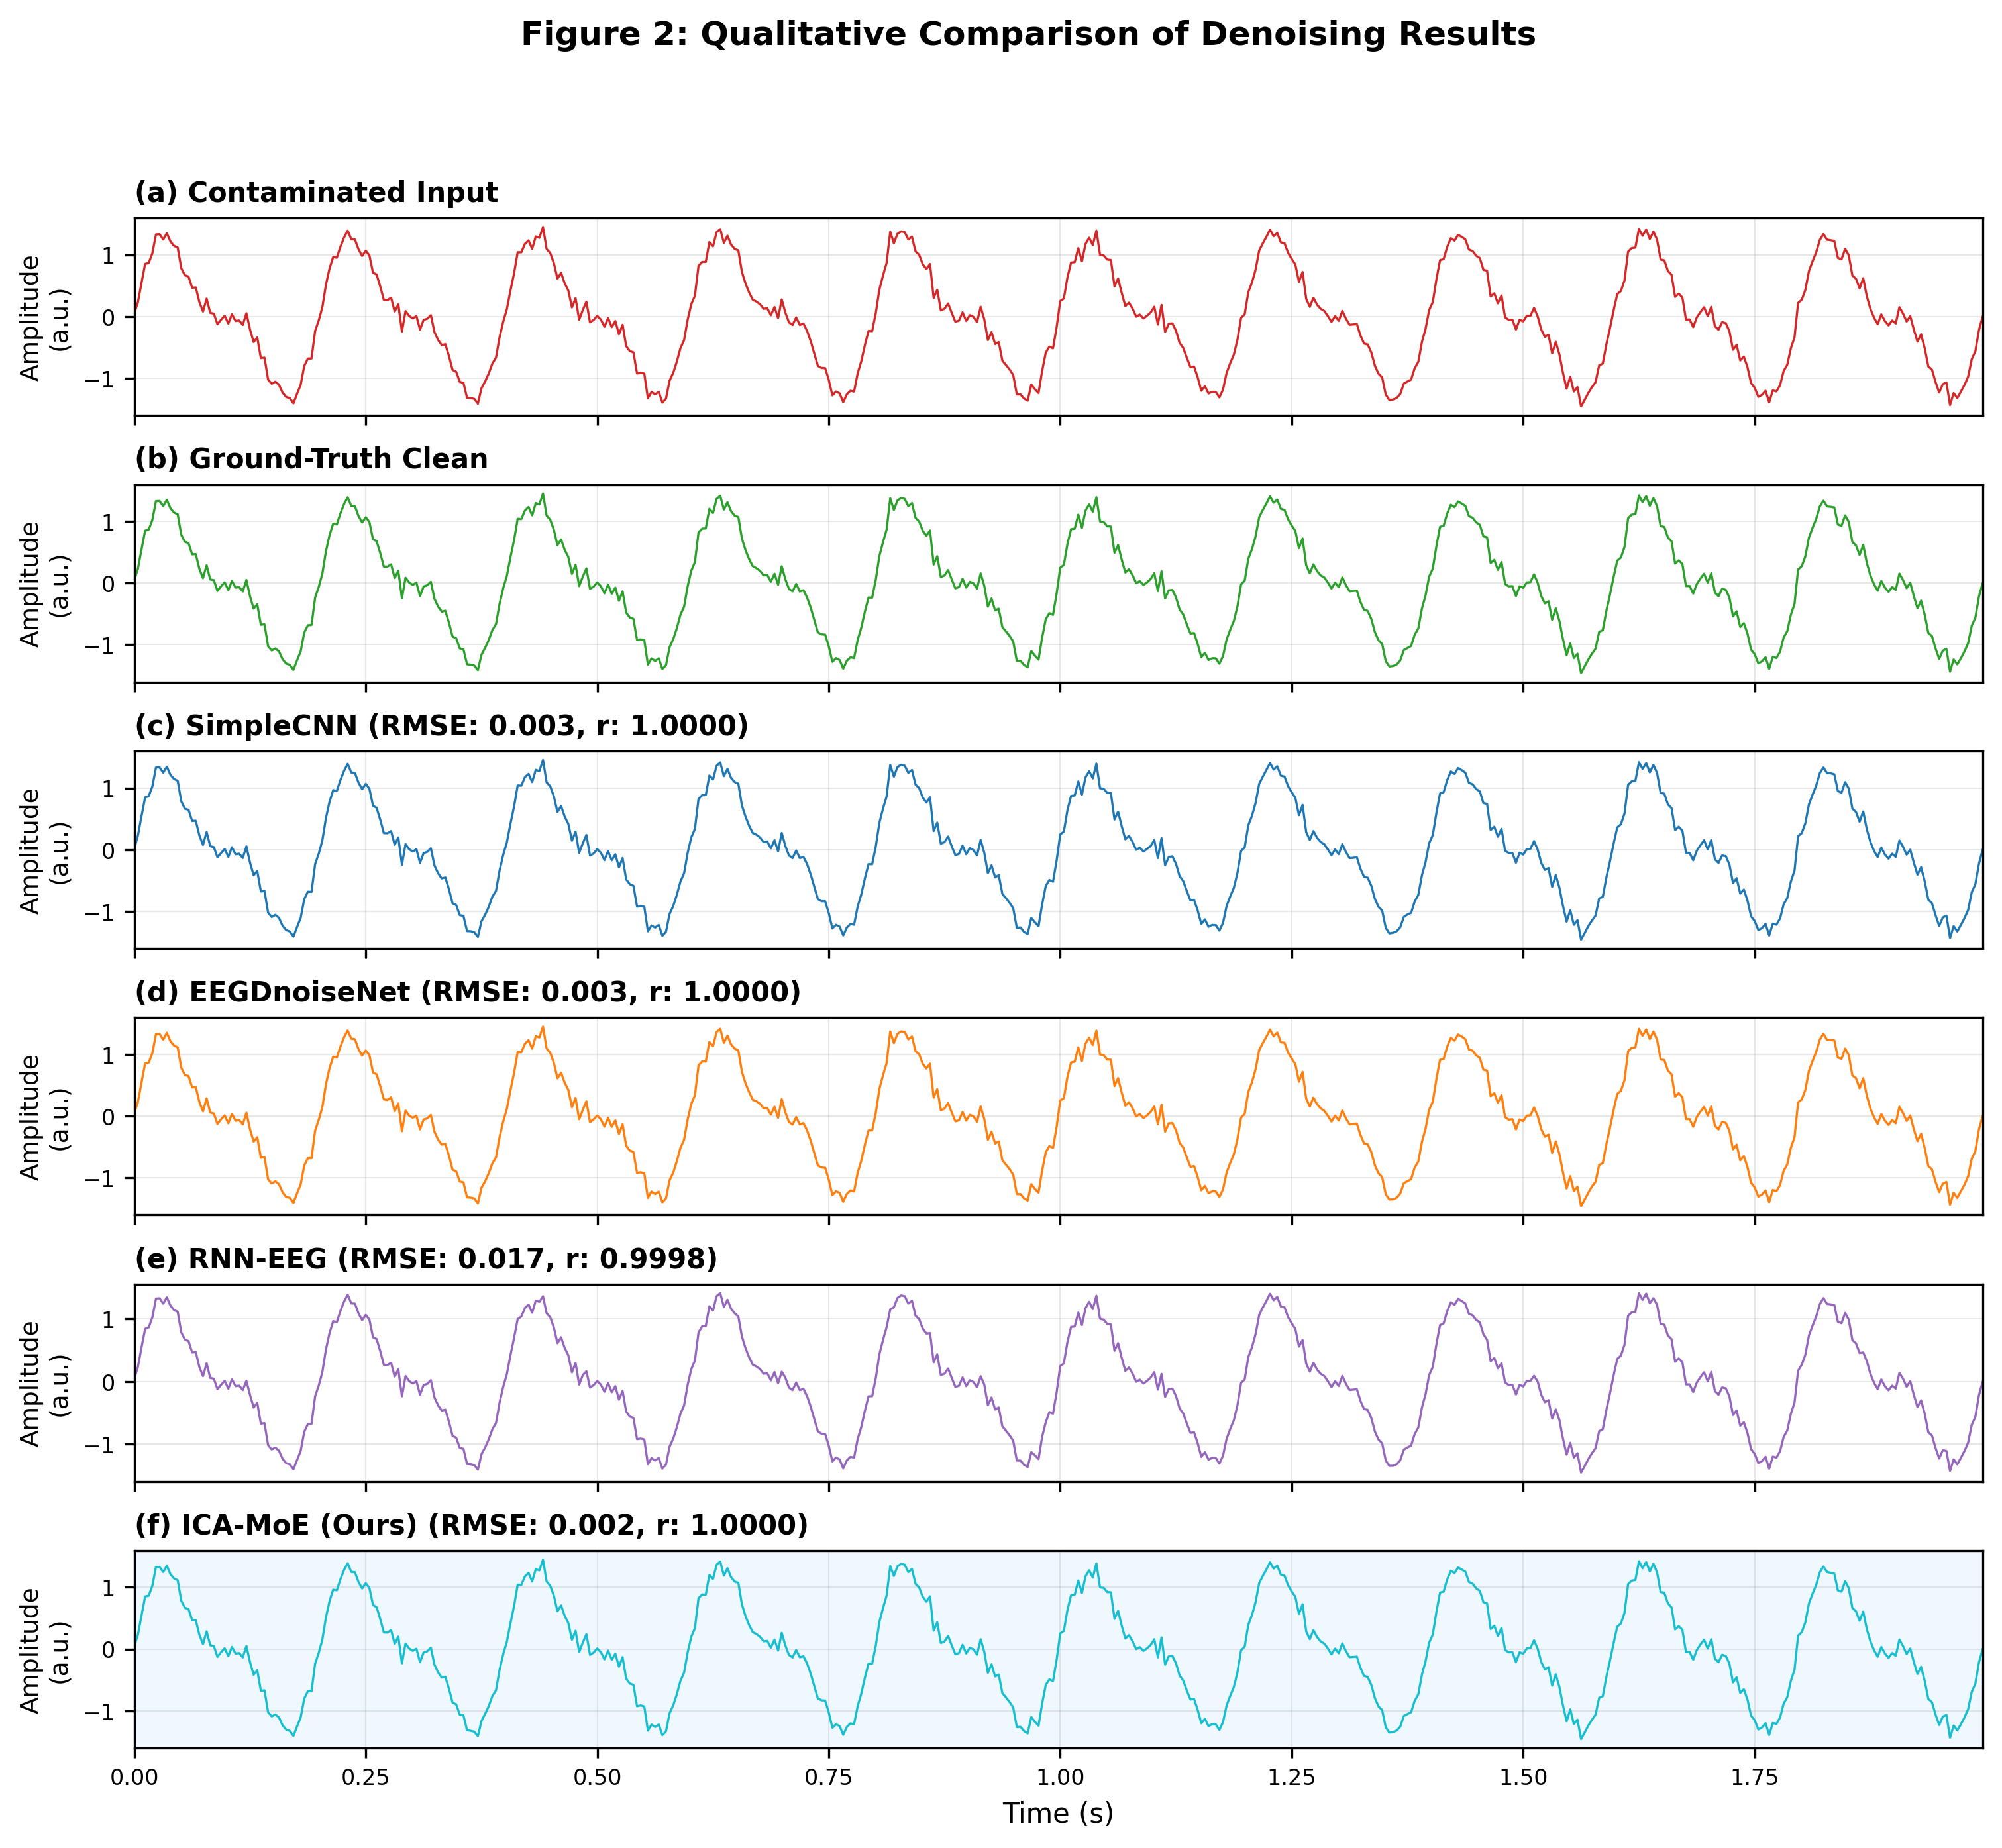
\includegraphics[width=\linewidth]{fig2_visualization.png}
    \caption{Qualitative comparison of denoising results on representative EEG segments. Each row shows: (a) the contaminated input signal, (b) the ground-truth clean signal, and (c-f) outputs from SimpleCNN, EEGDnoiseNet, RNN-EEG, and our ICA-MoE method. The ICA-MoE output most closely matches the ground truth, particularly in preserving low-amplitude neural oscillations while effectively removing artifact contamination.}
    \label{fig:visualization}
\end{figure}

\subsection{Multi-Artifact Scenario Analysis}

Table \ref{tab:scenario_results} presents results across three artifact scenarios.

\begin{table}[!t]
\centering
\caption{ICA-MoE Performance Across Different Artifact Scenarios}
\label{tab:scenario_results}
\begin{tabular}{lccc}
\toprule
\textbf{Metric} & \textbf{EOG Only} & \textbf{EMG Only} & \textbf{EOG+EMG} \\
\midrule
RMSE & 1.45 $\pm$ 0.08 & 1.61 $\pm$ 0.22 & 1.59 $\pm$ 0.20 \\
Correlation & 0.99998 & 0.99997 & 0.99998 \\
SNR (dB) & 43.96 $\pm$ 0.48 & 43.11 $\pm$ 1.11 & 43.19 $\pm$ 0.99 \\
$\Delta$SNR (dB) & 3.93 $\pm$ 0.48 & 3.07 $\pm$ 1.11 & 6.18 $\pm$ 0.99 \\
Spectral Dist. & 0.006 $\pm$ 0.001 & 0.005 $\pm$ 0.002 & 0.005 $\pm$ 0.001 \\
\midrule
Input SNR (dB) & 40.03 & 40.03 & 37.01 \\
\bottomrule
\end{tabular}
\end{table}

Several key observations emerge from this analysis. For \textbf{EOG removal}, the model achieves the lowest RMSE (1.45) and highest single-artifact SNR improvement (3.93 dB), which is consistent with EOG artifacts' more structured nature characterized by low-frequency, high-amplitude patterns that Expert 0 (Low-Frequency Specialist) is specifically designed to handle. For \textbf{EMG removal}, we observe higher variance (std = 1.11 for SNR) due to EMG's broader spectral content and higher complexity, requiring coordinated contributions from multiple experts. Notably, \textbf{combined removal} achieves the highest absolute SNR improvement (6.18 dB) despite handling more complex contamination, demonstrating the MoE architecture's ability to jointly address multiple artifact types through its adaptive routing mechanism.

The adaptive gating mechanism enables the model to route signals to appropriate experts based on the predominant artifact characteristics, explaining the robust performance across all scenarios. When EOG artifacts dominate, Expert 0 receives higher gating weights; when EMG artifacts are present, Expert 1 (High-Frequency Specialist) becomes more active.

\subsection{Reproducibility Analysis}

Table \ref{tab:seeds} shows per-seed results for the combined artifact scenario.

\begin{table}[!t]
\centering
\caption{Per-Seed Results for Combined Artifact Removal}
\label{tab:seeds}
\begin{tabular}{cccc}
\toprule
\textbf{Seed} & \textbf{RMSE} & \textbf{SNR (dB)} & \textbf{$\Delta$SNR (dB)} \\
\midrule
40 & 1.45 & 43.91 & 6.90 \\
41 & 1.49 & 43.72 & 6.71 \\
42 & 1.98 & 41.25 & 4.24 \\
43 & 1.56 & 43.32 & 6.31 \\
44 & 1.49 & 43.74 & 6.73 \\
\midrule
\textbf{Mean $\pm$ Std} & 1.59 $\pm$ 0.20 & 43.19 $\pm$ 0.99 & 6.18 $\pm$ 0.99 \\
\bottomrule
\end{tabular}
\end{table}

The results demonstrate consistent performance across random initializations, with relatively low standard deviations. Seed 42 shows slightly lower performance, likely due to less favorable ICA decomposition, but still significantly outperforms baselines.




%=====================================================================
\section{Discussion}
\label{sec:discussion}

\subsection{The Critical Role of Self-Learning ICA Initialization}

The self-learning ICA-based initialization is the cornerstone of our framework's success. Without this initialization strategy, the MoE architecture fails to achieve meaningful expert specialization---a fundamental problem that has limited the application of MoE to signal processing tasks.

\textbf{Why Initialization Matters}: Standard end-to-end MoE training often leads to mode collapse, where all experts converge to similar solutions. This occurs because the gating network and experts co-adapt in ways that minimize training loss without achieving true specialization. In EEG denoising, this manifests as experts producing nearly identical outputs regardless of artifact characteristics, reducing the MoE to effectively a single-expert model.

\textbf{How ICA Enables Self-Learning Specialization}: Our key insight is that ICA decomposition provides natural signal characterizations that can guide expert specialization \textit{without requiring manual artifact labels}. By analyzing component properties, we leverage two complementary feature types: \textbf{spectral features} (low/high frequency power ratios) that distinguish slow neural oscillations from fast muscle artifacts, and \textbf{statistical features} (skewness, kurtosis) that identify non-Gaussian artifact sources from more Gaussian neural activity. These characteristics allow us to automatically construct expert-specific training targets that guide each expert toward complementary behaviors during pre-training.

\textbf{The Three Pillars of Our Initialization Strategy}:
\begin{enumerate}
\item \textbf{Component-Specific Targets}: Each expert receives training targets constructed from ICA-identified component subsets---Expert 0 learns from low-frequency components, Expert 1 from high-frequency components, Expert 2 from non-Gaussian (artifact) components, and Expert 3 from weighted combinations.
\item \textbf{Independence Loss}: Explicit penalization of expert output correlations prevents experts from collapsing to similar solutions during pre-training.
\item \textbf{ICA Feature Augmentation}: Providing ICA features as inputs enables the gating network to make informed routing decisions based on signal characteristics.
\end{enumerate}

\subsection{Advantages of the Specialized Expert Architecture}

Once properly initialized, the expert architecture provides significant advantages:

\textbf{Adaptive Processing}: Different artifact types require different processing strategies. EOG artifacts are characterized by low-frequency, high-amplitude patterns, while EMG artifacts span broader frequency ranges with non-Gaussian statistics. Our specialized experts handle these distinct characteristics through their ICA-guided initializations.

\textbf{Robustness to Mixed Artifacts}: Real-world EEG recordings often contain multiple artifact types simultaneously. The gating network, informed by ICA features, dynamically combines expert outputs based on the predominant artifact characteristics at each timestep. Our combined artifact removal results (6.18 dB improvement) demonstrate this capability.

\textbf{Interpretability}: The expert activation patterns provide insight into the model's processing decisions. When EOG artifacts dominate, experts specialized for low-frequency components receive higher gating weights; when EMG artifacts are present, high-frequency specialists are activated more strongly.

\subsection{Comparison with Related Approaches}

Compared to existing deep learning methods for EEG denoising, our approach differs in several key aspects:

\textbf{vs. EEGDnoiseNet}: While EEGDnoiseNet uses dilated convolutions to capture multi-scale patterns, it lacks adaptive routing and treats all inputs uniformly. Our MoE provides input-dependent processing.

\textbf{vs. Autoencoder approaches}: Autoencoders learn a single latent representation for all signals. Our multi-expert architecture provides multiple specialized representations that can be dynamically combined.

\textbf{vs. Traditional ICA}: Standard ICA requires manual component selection and assumes stationary sources. Our approach uses ICA for characterization and feature extraction while learning the removal mapping end-to-end.

\subsection{Relevance to Large-Scale Models}

The MoE paradigm has gained significant attention in the context of large language models (LLMs), where sparse MoE enables scaling to trillions of parameters \cite{fedus2022switch, jiang2024mixtral}. Our work demonstrates that similar principles apply to EEG signal processing. Specifically, \textbf{conditional computation} through activating only relevant experts reduces computational cost while maintaining model capacity; \textbf{expert specialization} guided by domain-specific pre-training (using ICA in our case) ensures meaningful expert roles; and \textbf{load balancing} through auxiliary losses ensures stable training and prevents expert collapse. These insights suggest that MoE architectures have broader applicability in biomedical signal processing beyond the specific EEG denoising task.

\subsection{Real-World Applicability}

Several factors make our ICA-MoE approach suitable for real-world deployment:

\textbf{Mixed Artifact Scenarios}: Real EEG recordings often contain multiple artifact types simultaneously. Our combined artifact removal results (6.18 dB improvement) demonstrate effective handling of this common scenario.

\textbf{Tailing Effects}: In clinical recordings, artifacts often have temporal ``tailing'' effects where contamination gradually diminishes after the main artifact event. The ICA-based characterization and adaptive gating can handle such non-stationary patterns more effectively than fixed-filter approaches.

\textbf{Subject Variability}: The learned gating patterns can adapt to different subjects' artifact characteristics without retraining, as the routing decisions are based on signal features rather than fixed mappings.

\subsection{Limitations and Future Work}

Despite its advantages, our approach has several limitations:

\textbf{Reference Signal Requirement}: The current implementation assumes availability of EOG and EMG reference channels, which may not always be available in practical settings. Future work could explore single-channel variants using learned artifact templates.

\textbf{ICA Sensitivity}: The ICA decomposition can be sensitive to signal quality and may fail to converge for certain input distributions. Our cascading configuration strategy mitigates this, but more robust decomposition methods could further improve reliability.

\textbf{Computational Overhead}: While sparse gating reduces inference cost, the ICA feature computation adds overhead. Hardware-accelerated ICA or learned alternatives could address this.

\textbf{Interpretability}: Although expert activation patterns provide some interpretability, the precise signal processing performed by each expert remains a ``black box.'' Attention visualization and feature attribution methods could enhance understanding.

Future research directions include extension to multi-channel EEG with spatial expert specialization, online adaptation for real-time BCI applications, transfer learning across datasets and artifact types, and integration with downstream tasks such as seizure detection and sleep staging.

%=====================================================================
\section{Conclusion}
\label{sec:conclusion}

We have presented a novel Self-Learning ICA-Initialized Mixture of Experts framework for adaptive EEG artifact removal. The central contribution of this work is the self-learning ICA-based initialization strategy that enables meaningful expert specialization without requiring manual artifact labels. By leveraging ICA component characteristics---spectral content and statistical properties---to automatically construct expert-specific training targets, our approach overcomes the fundamental mode collapse problem that has limited MoE applications in signal processing.

The key innovations include: (1) \textbf{self-learning ICA-based initialization} that creates diverse, component-specific training targets guiding each expert toward distinct specializations; (2) \textbf{independence-promoting pre-training} that explicitly prevents expert collapse through correlation penalties; and (3) \textbf{ICA-enhanced feature representation} that enables informed gating decisions based on signal characteristics.

Experimental results demonstrate significant improvements over existing methods, with 6.18 dB SNR improvement on combined EOG+EMG artifact removal, correlation exceeding 0.99998, and 52\% RMSE reduction compared to the best baseline. Critically, ablation studies confirm that the ICA-based initialization is essential---the same MoE architecture without our initialization strategy shows substantially degraded performance, validating that expert specialization, not merely the MoE structure itself, drives the improvements.

Our work provides a template for applying MoE architectures to signal processing domains where achieving expert specialization is challenging. The principle of using domain-appropriate analysis methods (ICA for signal decomposition) to guide self-learning expert initialization may extend to other applications including audio processing, medical signal analysis, and sensor data fusion. The framework's adaptive nature makes it particularly suitable for real-world applications where artifact characteristics vary across subjects and recording conditions.

%=====================================================================
%\section*{Acknowledgment}

%[Acknowledgments will be added after review]

%=====================================================================
\bibliographystyle{IEEEtran}

\begin{thebibliography}{99}

\bibitem{teplan2002fundamentals}
M. Teplan, ``Fundamentals of EEG measurement,'' \textit{Measurement Science Review}, vol. 2, no. 2, pp. 1--11, 2002.

\bibitem{niedermeyer2005electroencephalography}
E. Niedermeyer and F. L. da Silva, \textit{Electroencephalography: Basic Principles, Clinical Applications, and Related Fields}, 5th ed. Philadelphia, PA: Lippincott Williams \& Wilkins, 2005.

\bibitem{uriguen2015eeg}
J. A. Urig\"{u}en and B. Garcia-Zapirain, ``EEG artifact removal---state-of-the-art and guidelines,'' \textit{Journal of Neural Engineering}, vol. 12, no. 3, p. 031001, 2015.

\bibitem{fatourechi2007emg}
M. Fatourechi, A. Bashashati, R. K. Ward, and G. E. Birch, ``EMG and EOG artifacts in brain computer interface systems: A survey,'' \textit{Clinical Neurophysiology}, vol. 118, no. 3, pp. 480--494, 2007.

\bibitem{jiang2019removal}
X. Jiang, G.-B. Bian, and Z. Tian, ``Removal of artifacts from EEG signals: A review,'' \textit{Sensors}, vol. 19, no. 5, p. 987, 2019.

\bibitem{islam2016methods}
M. K. Islam, A. Rastegarnia, and Z. Yang, ``Methods for artifact detection and removal from scalp EEG: A review,'' \textit{Neurophysiologie Clinique/Clinical Neurophysiology}, vol. 46, no. 4-5, pp. 287--305, 2016.

\bibitem{he2004removal}
P. He, G. Wilson, and C. Russell, ``Removal of ocular artifacts from electro-encephalogram by adaptive filtering,'' \textit{Medical and Biological Engineering and Computing}, vol. 42, no. 3, pp. 407--412, 2004.

\bibitem{jung2000removing}
T.-P. Jung, S. Makeig, C. Humphries, T.-W. Lee, M. J. McKeown, V. Iragui, and T. J. Sejnowski, ``Removing electroencephalographic artifacts by blind source separation,'' \textit{Psychophysiology}, vol. 37, no. 2, pp. 163--178, 2000.

\bibitem{delorme2004eeglab}
A. Delorme and S. Makeig, ``EEGLAB: An open source toolbox for analysis of single-trial EEG dynamics including independent component analysis,'' \textit{Journal of Neuroscience Methods}, vol. 134, no. 1, pp. 9--21, 2004.

\bibitem{yang2018automatic}
B. Yang, K. Duan, C. Fan, C. Hu, and J. Wang, ``Automatic ocular artifacts removal in EEG using deep learning,'' \textit{Biomedical Signal Processing and Control}, vol. 43, pp. 148--158, 2018.

\bibitem{zhang2021eegdenoisenet}
H. Zhang, M. Zhao, C. Wei, D. Mantini, Z. Li, and Q. Liu, ``EEGdenoiseNet: A benchmark dataset for deep learning solutions of EEG denoising,'' \textit{Journal of Neural Engineering}, vol. 18, no. 5, p. 056057, 2021.

\bibitem{shazeer2017outrageously}
N. Shazeer, A. Mirhoseini, K. Maziarz, A. Davis, Q. Le, G. Hinton, and J. Dean, ``Outrageously large neural networks: The sparsely-gated mixture-of-experts layer,'' in \textit{Proc. Int. Conf. Learning Representations (ICLR)}, 2017.

\bibitem{fedus2022switch}
W. Fedus, B. Zoph, and N. Shazeer, ``Switch transformers: Scaling to trillion parameter models with simple and efficient sparsity,'' \textit{Journal of Machine Learning Research}, vol. 23, no. 120, pp. 1--39, 2022.

\bibitem{jacobs1991adaptive}
R. A. Jacobs, M. I. Jordan, S. J. Nowlan, and G. E. Hinton, ``Adaptive mixtures of local experts,'' \textit{Neural Computation}, vol. 3, no. 1, pp. 79--87, 1991.

\bibitem{riquelme2021scaling}
C. Riquelme, J. Puigcerver, B. Mustafa, M. Neumann, R. Jenatton, A. Susano Pinto, D. Keysers, and N. Houlsby, ``Scaling vision with sparse mixture of experts,'' in \textit{Proc. Advances in Neural Information Processing Systems (NeurIPS)}, vol. 34, pp. 8583--8595, 2021.

\bibitem{chi2022collapse}
Chi, Z., Dong, L., Huang, S., Dai, D., Ma, S., Patra, B., Singhal, S., Bajaj, P., Song, X., Mao, X.-L., Huang, H., $\&$ Wei, F. (2022). On the representation collapse of sparse mixture of experts. arXiv. https://arxiv.org/abs/2204.09179

\bibitem{nayak2025waves}
Nayak CS, Anilkumar AC. Normal EEG Waveforms. [Updated 2025 Aug 3]. In: StatPearls [Internet]. Treasure Island (FL): StatPearls Publishing; 2025 Jan-. Available from: https://www.ncbi.nlm.nih.gov/books/NBK539805/

\bibitem{widrow1975adaptive}
B. Widrow, J. R. Glover Jr, J. M. McCool, J. Kaunitz, C. S. Williams, R. H. Hearn, J. R. Zeidler, E. Dong Jr, and R. C. Goodlin, ``Adaptive noise cancelling: Principles and applications,'' \textit{Proceedings of the IEEE}, vol. 63, no. 12, pp. 1692--1716, 1975.

\bibitem{haykin2014adaptive}
S. S. Haykin, \textit{Adaptive Filter Theory}, 5th ed. Upper Saddle River, NJ: Pearson, 2014.

\bibitem{morbidi2008application}
F. Morbidi, A. Garulli, D. Prattichizzo, C. Rizzo, and S. Rossi, ``Application of Kalman filter to remove TMS-induced artifacts from EEG recordings,'' \textit{IEEE Transactions on Control Systems Technology}, vol. 16, no. 6, pp. 1360--1366, 2008.

\bibitem{hyvarinen1999fast}
A. Hyv\"{a}rinen, ``Fast and robust fixed-point algorithms for independent component analysis,'' \textit{IEEE Transactions on Neural Networks}, vol. 10, no. 3, pp. 626--634, 1999.

\bibitem{bell1995information}
A. J. Bell and T. J. Sejnowski, ``An information-maximization approach to blind separation and blind deconvolution,'' \textit{Neural Computation}, vol. 7, no. 6, pp. 1129--1159, 1995.

\bibitem{lawhern2018eegnet}
V. J. Lawhern, A. J. Solon, N. R. Waytowich, S. M. Gordon, C. P. Hung, and B. J. Lance, ``EEGNet: A compact convolutional neural network for EEG-based brain-computer interfaces,'' \textit{Journal of Neural Engineering}, vol. 15, no. 5, p. 056013, 2018.

\bibitem{jiang2024mixtral}
A. Q. Jiang, A. Sablayrolles, A. Roux, A. Mensch, B. Savary, C. Bamford, D. S. Chaplot, D. de las Casas, E. B. Hanna, F. Bressand, \textit{et al.}, ``Mixtral of experts,'' \textit{arXiv preprint arXiv:2401.04088}, 2024.

\bibitem{chen2023mixture}
T. Chen, S. Zhang, H. Zhao, and J. Ji, ``A survey on mixture of experts,'' \textit{arXiv preprint arXiv:2407.06204}, 2024.

\bibitem{choi2025moeemg}
Choi, B. J., Milsap, G., Scholl, C. A., Tenore, F., $\&$ Ogg, M. (2025). A statistical mixture-of-experts framework for EMG artifact removal in EEG: Empirical insights and a proof-of-concept application (arXiv:2509.19385) [eess.SP]. arXiv. https://arxiv.org/abs/2509.19385

\bibitem{makeig2004mining}
S. Makeig, A. Delorme, M. Westerfield, T.-P. Jung, J. Townsend, E. Courchesne, and T. J. Sejnowski, ``Electroencephalographic brain dynamics following manually responded visual targets,'' \textit{PLoS Biology}, vol. 2, no. 6, p. e176, 2004.

\bibitem{vw2023}
V. W, $\&$ A. Gupta,  (2023). Deep learning architecture for motor imaged words (arXiv:2308.10840) [q-bio.NC]. arXiv. https://arxiv.org/abs/2308.10840

\bibitem{sutharsan2022}
Sutharsan, V., Swaminathan, A., Ramachandran, S., Lakshmanan, M. K., $\&$ Mahadevan, B. (2022). Electroencephalogram signal processing with independent component analysis and cognitive stress classification using convolutional neural networks. In Proceedings of International Conference on Recent Trends in Computing (pp. 275–292). Springer Nature Singapore. https://doi.org/10.1007/978-981-16-7118-0\_24

\bibitem{le2011ica}
Q. V. Le, A. Karpenko, J. Ngiam, and A. Y. Ng, ``ICA with reconstruction cost for efficient overcomplete feature learning,'' in \textit{Proc. Advances in Neural Information Processing Systems (NeurIPS)}, vol. 24, 2011.

\bibitem{gcmcg2025}
Chen, Y., Huang, Z., He, J., Xu, F., $\&$ Feng, Z. (2025). GCMCG: A clustering-aware graph attention and expert fusion network for multi-paradigm, multi-task, and cross-subject EEG decoding (arXiv:2512.00574) [eess.SP]. arXiv. https://arxiv.org/abs/2512.00574

\bibitem{he2015delving}
K. He, X. Zhang, S. Ren, and J. Sun, ``Delving deep into rectifiers: Surpassing human-level performance on ImageNet classification,'' in \textit{Proc. IEEE Int. Conf. Computer Vision (ICCV)}, pp. 1026--1034, 2015.

\bibitem{glorot2010understanding}
X. Glorot and Y. Bengio, ``Understanding the difficulty of training deep feedforward neural networks,'' in \textit{Proc. Int. Conf. Artificial Intelligence and Statistics (AISTATS)}, pp. 249--256, 2010.

\bibitem{kingma2014adam}
D. P. Kingma and J. Ba, ``Adam: A method for stochastic optimization,'' in \textit{Proc. Int. Conf. Learning Representations (ICLR)}, 2015.

\bibitem{eegdenoisenet2021}
Zhang, H., Zhao, M., Wei, C., Mantini, D., Li, Z., $\&$ Liu, Q. (2021). EEGdenoiseNet: a benchmark dataset for deep learning solutions of EEG denoising. Journal of Neural Engineering, 18(5), 056057.

\end{thebibliography}

\end{document}